\section{Communication System}
\subsection{overview}
There are the most important components in  a fiber communication system (see Figure [\ref{flow-chart}]): 
\begin{enumerate}
\item Transmitter: turn a complex symbol sequence to a wave form signal and transmitted to a fiber channel.
$$
\{X_n\}_{n=0}^{N} \rightarrow u(0,t), t\in R^{+}
$$
Where $X_n\in \mathbb{C}$ are the transmmited symbols, $u \in \mathbb{C}$ is the wave form signal. We assume total N symbols here.
\item Fiber channel: evolution the analog signal from $z=0$ to $z=L$.
$$
 u(0,t) \rightarrow u(L,t)
$$
\item Reciever: sampled data points from the received signal $u(L,t)$ and turn this data to a complex symbol sequence. 
$$
u(L,t) \rightarrow \{Y_n\}_{n=0}^{N}
$$ 
where $Y_n \in \mathbb{C}$ is output symbols.
\end{enumerate}
\begin{figure}[ht]
\centering
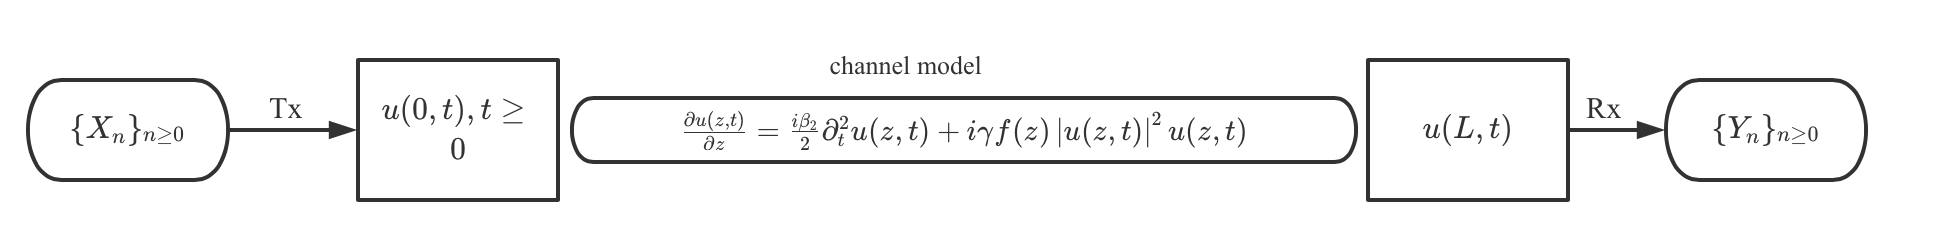
\includegraphics[width=\linewidth]{img/flow-chart.png}
\caption{data flow}
\label{flow-chart}
\end{figure}
Because of the noise in fiber channel, we get a channel conditional probability:
$$
P(Y|X)
$$
where $X = (X_1,X_2,\ldots,X_N)$, $Y=(Y_1,Y_2,\ldots,Y_N)$.\\
\textbf{Our target}
\begin{enumerate}
\item In practice. We want to increase the bit error rate(BER) as much as we can.
$$
BER = Pr(X_n=Y_n)
$$
\item In theorem. We want to know the capacity limit in such a nonlinear communication system.
\begin{align*}
C = \sup\limits_{P(X)} \frac{1}{N}I(X:Y)
\end{align*}
Here $I(X;Y)$ is the mutual information between two random vectors. This formula is the famous Seccond shannon theorem.
\end{enumerate}


\subsection{Transmitter Model}

\begin{equation}\label{Tx}
\left\{
\begin{aligned}
& u(0,t) = \sum_{i=M}^{-M} A_i(0,t) exp(i (\omega_i - \omega_0) t) & t\in [0,T_f]\\
& A_i(0,t) = \sqrt{P_i}\sum_{k=0}^{N-1} x^i_k g(t - kT) \\
\end{aligned}
\right.
\end{equation}
Where $g(t)$ is the Raise-Cosin signal pulse controled by a roll-off parameter $\beta$. Show as formula (\ref{pulse}) and figure (\ref{Raise-Cosin}). $T$ is symbol period and $T_f = N*T$ is the signal length. $P_0$ is the peak power. $x^i_k \in \mathbb{C}$ is complex symbol (See Remark (\ref{4QAM})). $\omega_0$ is the central carrier frenquency.

\begin{remark}\label{4QAM}
[4QAM]
$$
x^k_j \in \mathcal{X} = \{\pm 1 \pm i \}
$$
\begin{figure}[htbp]
\centering
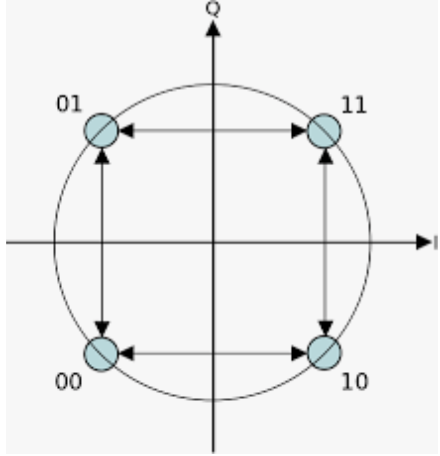
\includegraphics[width=0.2\linewidth]{img/4QAM.png}
\end{figure}
\end{remark}

\begin{equation}\label{pulse}
g(t)=\left\{\begin{array}{ll}
\frac{\pi}{4 T} \operatorname{sinc}\left(\frac{1}{2 \beta}\right), & t=\pm \frac{T}{2 \beta} \\
\frac{1}{T} \operatorname{sinc}\left(\frac{t}{T}\right) \frac{\cos \left(\frac{\pi \beta t}{T}\right)}{1-\left(\frac{2 \beta t}{T}\right)^{2}}, & \text { otherwise }
\end{array}\right.
\end{equation}

\begin{figure}[htbp]
\centering
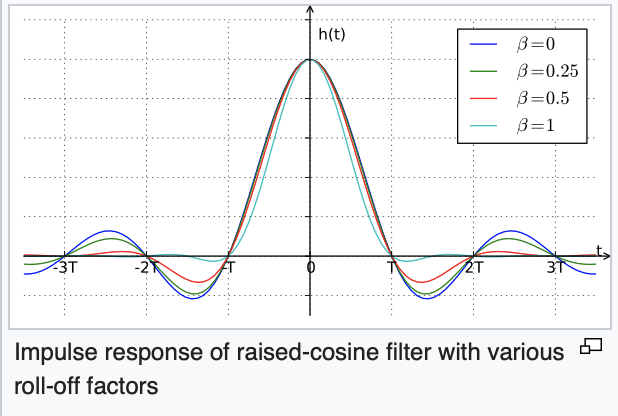
\includegraphics[width=0.3\linewidth]{img/rc_t.png}
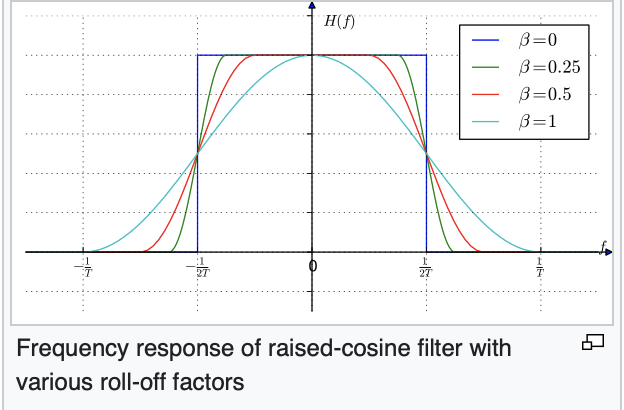
\includegraphics[width=0.3\linewidth]{img/rc_f.png}
\caption{Raise-Cosin signal pulse}
\label{Raise-Cosin}
\end{figure}


\subsection{Fiber model}
\subsubsection{Nonlinear Schrodinger equation model (NLSE)}
\begin{equation}\label{model}
\left\{
\begin{aligned}
& \frac{\partial u(z, t)}{\partial z}=-\frac{\alpha}{2}u(z,t) + \frac{i\beta_2}{2} \frac{\partial^2 u(z,t)}{\partial t^2} + i \gamma \left|u(z, t)\right|^{2} u(z, t) + n(z,t) \\
& u(z,0) = u(z,T_f) \\
& u(0,t) = \sum_{i=M}^{-M} A_i(0,t) exp(i (\omega_i - \omega_0) t) \\
& A_i(0,t) = \sqrt{P_i}\sum_{k=1}^{N} x^i_k g(t - kT) \\
& (z,t) \in [0,L] \times [0,T_f]
\end{aligned}
\right.
\end{equation}
Where $\alpha$,$\beta_2$,$\gamma$ denote attenuation, group velocity dispersion, and fiber nonlinearity coefficient.  $n(z,t)$ is a complex Gaussian noise process with autocorrelation (\ref{noise})(see \cite{path_int}). 
\begin{remark}\label{noise}
[noise term]
\begin{equation}
\left\{
\begin{aligned}
& \left\langle n(z, \omega) \bar{n}\left(z^{\prime}, \omega^{\prime}\right)\right\rangle_{n}=2 \pi \mathcal{Q} \delta\left(\omega-\omega^{\prime}\right) \theta\left(\frac{W^{\prime}}{2}-|\omega|\right) \delta\left(z-z^{\prime}\right) \\
& \left\langle n(z, t) \bar{n}\left(z^{\prime}, t^{\prime}\right)\right\rangle_{n}=\frac{\mathcal{Q}}{\pi\left(t-t^{\prime}\right)} \sin \left(\frac{W^{\prime}\left(t-t^{\prime}\right)}{2}\right) \delta\left(z-z^{\prime}\right)
\end{aligned}
\right.
\end{equation}

Where $\theta(x)$ is Heaviside theta-function. 

\end{remark}


\begin{remark}
[FT]
$$
n(z, \omega)=\int_{-\infty}^{\infty} d t e^{-i \omega t} n(z, t)
$$
\end{remark}



\subsubsection{Couple Nonlinear Schrodinger Equation model (CNLSE)}
Use the WDM initial expression (\ref{WDM initial value}), and neglect FWM terms(when can we neglect this term ?), we can get a simpler model (\ref{CNLSE}).
\begin{equation}\label{WDM initial value}
u(z,t) = \sum_{i=M}^{-M} A_i(z,t) exp(i (\omega_i - \omega_0) t)
\end{equation}

\begin{equation}\label{CNLSE}
\frac{\partial A_i(z, t)}{\partial z}=-\frac{\alpha}{2}A_i(z,t)-\beta_{i1}\frac{\partial A_i(z,t)}{\partial t} + \frac{i\beta_{i2}}{2} \frac{\partial^2 A_i(z,t)}{\partial t^2} + i \gamma \left(|A_i|^{2} + 2\sum_{q\neq i} |A_q|^2\right) A_i(z, t) + n(z,t)
\end{equation}

\subsubsection{Split Step Fourier Method}
To solve the NLSE and CNLSE, we review the classical Split Step Fourier Method(SSFM) .
\begin{figure}[htbp]
\centering
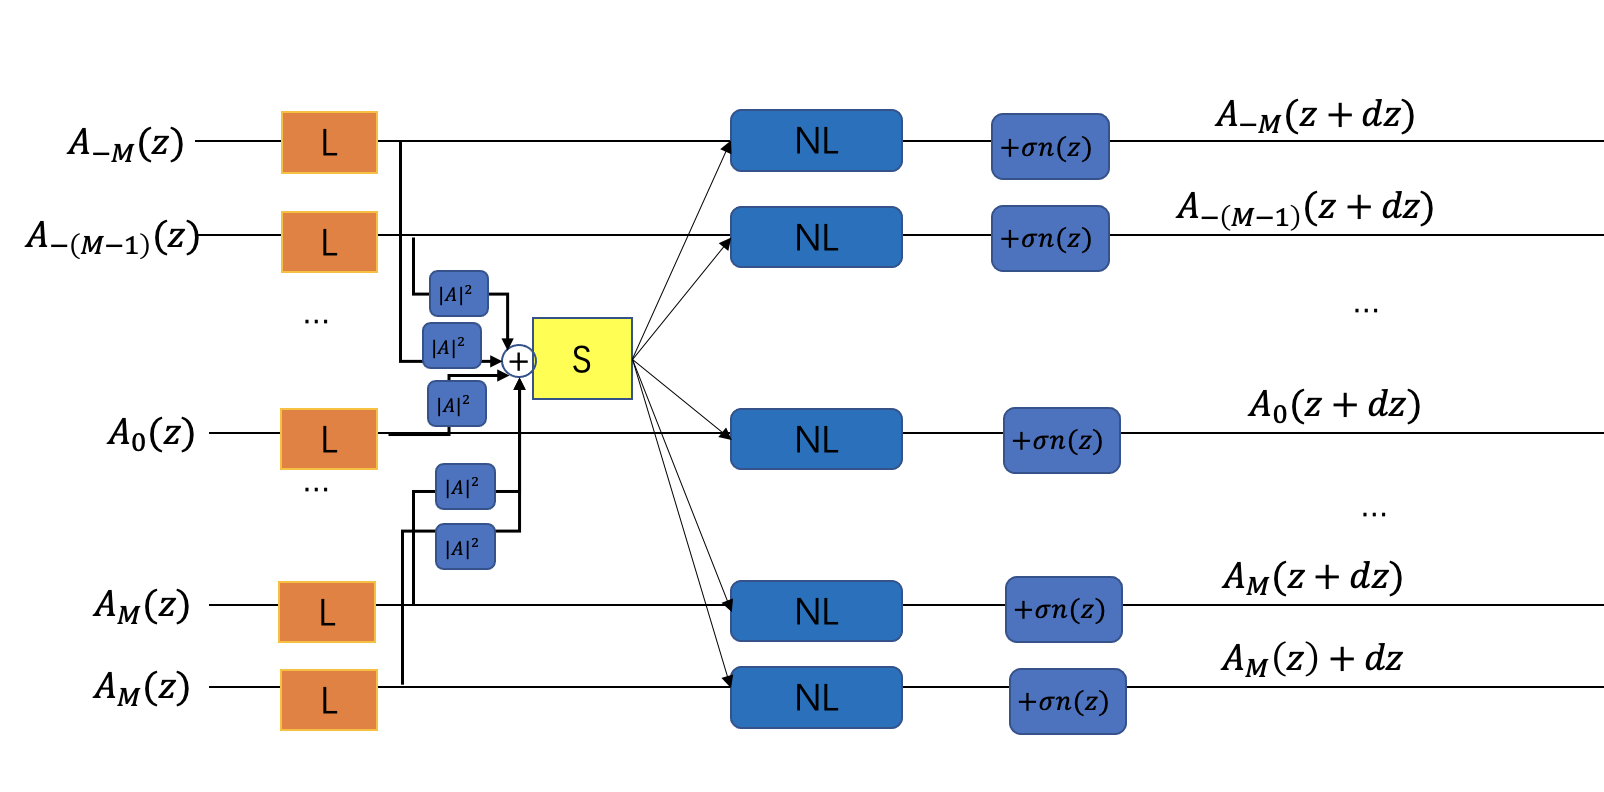
\includegraphics[width=0.6\linewidth]{img/SSFM.png}
\caption{SSFM structure: one step}
\label{SSFM fig}
\end{figure}
$$
SSFM: \left(\begin{array}{c}A_{-M}(0,t)\\A_{-(M-1)}(0,t)\\\ldots\\A_{0}(0,t)\\\ldots\\A_{M}(0,t)\end{array}\right) \rightarrow\left(\begin{array}{c}A_{-M}(L,t)\\A_{-(M-1)}(L,t)\\\ldots\\A_{0}(L,t)\\\ldots\\A_{M}(L,t)\end{array}\right)
$$
Using SSMF method: Linar step and Nonlinear step alternate. Assume each symbol take $N_t$ points sampling at equal intervals. Define collocation points $t_j = j\frac{T}{N_t} (0\leq j \leq N_{f})$. Here, $N_{f} = N*N_t$. 
\begin{align*}
A_i(z) := [A_i(z,t_0), A_i(z,t_1),\ldots,A_i(z,t_{N_{f}})] \in \mathbb{C}^{N_{f}} \\
\end{align*}
The transfer function:
\begin{align*}
& \mathbf{\omega} = \frac{2\pi}{T_f}[0,1,\ldots,\frac{N_f}{2},-\frac{N_f}{2}+1,-\frac{N_f}{2}+2,\ldots,-1] \in \mathbb{C}^{N_f}\\
& H_i(dz) = \exp \left[\left(-\frac{\alpha}{2} - \mathrm{i}\beta_{i1} \mathbf{\omega} - \mathrm{i} \beta_{i2} \frac{\mathbf{\omega}^{2}}{2}\right) dz\right] \in \mathbb{C}^{N_f}
\end{align*}
\begin{enumerate}
\item Linear step
\begin{equation}\label{linear step}
A_i(z + dz) = L_{H_i(dz)}(A_i(z)) := ifft(fft(A_i(z)) .* H_i(dz))
\end{equation}
\item Nonlinear step
\begin{equation}\label{nonlinear step}
A_i(z+dz) = NL_{dz,S_i} (A_i(z)) := A_i(z) .* \exp\left(\mathrm{i} \gamma dz * (S_i+|A_i|^2)\right) := A_i(z) .* \exp\left(i \gamma dz * (2\sum_{q\neq i} |A_q(z)|^2+|A_i(z)|^2)\right)
\end{equation}
We use $S_i$ to denotes the power sum of the other channels.
\begin{equation}\label{define S}
S_i = 2\sum_{q\neq i} |A_q(z)|^2
\end{equation}
\end{enumerate}

\begin{algorithm}[t]
\caption{SSFM} %算法的名字
\hspace*{0.02in} {\bf Input:} %算法的输入, \hspace*{0.02in}用来控制位置,同时利用 \\ 进行换行
input transmmitted signals $A_i(0)(-M \leq i \leq M)$, step size $dz$, noise level $\sigma$,transmmitted length $L$\\
\hspace*{0.02in} {\bf Output:} %算法的结果输出
output result
\begin{algorithmic}[1]
\State $K = \frac{L}{dz}$  % \State 后写一般语句
\For{s = 1,...,K} % For 语句,需要和EndFor对应
   \State Linear step:
        $$
        A_i^{1}(z) = L_{H_i(dz)}(A_i(z))
        $$
    \State Calculate $S_i$:
        $$
        S_i = 2\sum_{q\neq i} |A_i^1(z)|^2
        $$
    \State Nonlinear step:
        $$
        A_i^2(z) = NL_{dz,S_i}(A^1_i(z))
        $$
    \State Add noise: sample a gaussian noise $n(z)$.
        $$
            A_i(z+dz) \leftarrow A_i(z+dz) + \sigma * n(z)
        $$
    \State $z \leftarrow z + dz$
\EndFor
\State \Return $A_i(L)$, $-M \leq i \leq M$
\end{algorithmic}
\end{algorithm}
The whole process show in Figure [\ref{SSFM fig}].

\subsection{Receiver Model}
There are three steps in our receiver model.
\begin{enumerate}
\item Digital back propagation. This step is the most import part to compensate all kinds of interference. We will design some algorithm in Section 2.
    \begin{equation}\label{DBP}
    \hat{A}_0(t) = DBP(A_0(L,t))
    \end{equation}
\item Filter.
    \begin{equation}
    \tilde{x}_k^0 = \frac{1}{\sqrt{P_0} \|g\|_2^2}\int_{-\infty}^{+\infty} \hat{A}_0(t) g_k(t) dt
    \end{equation}
    Here we define $g_k(t) = g(t - kT)$, then $g_k$ is othorgonal with respect to diffrent $k$.
\item Classification.
    \begin{equation}
    \hat{x}_k^0 = \mathop{argmin}\limits_{x\in \mathcal{X}} \|x - \tilde{x}_k^0\|
    \end{equation}
\end{enumerate}
We can show the whole communication system as Figure \ref{communication system}.

\begin{figure}[htbp]
\centering
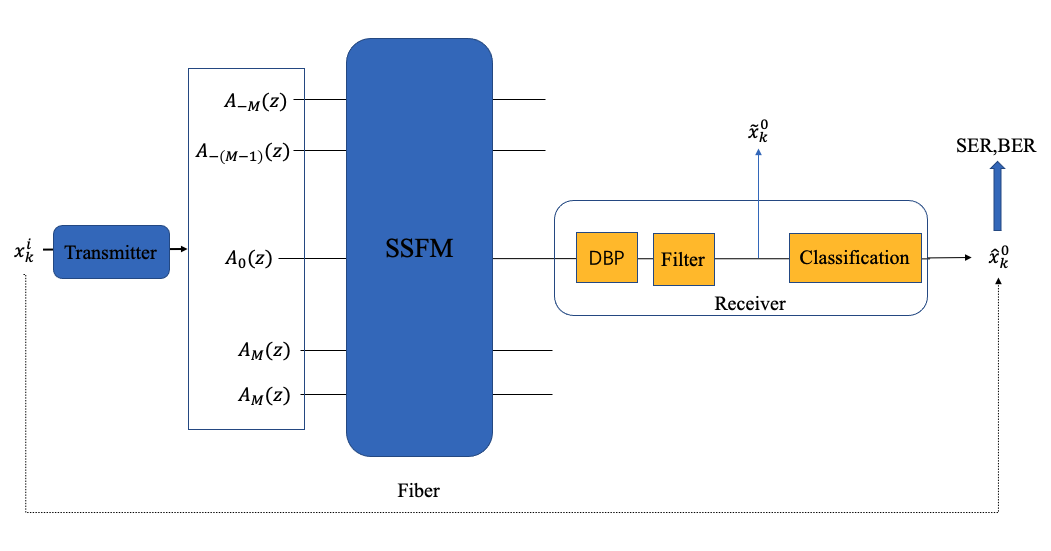
\includegraphics[width=0.8\linewidth]{img/com_system.png}
\caption{communication system}
\label{communication system}
\end{figure}













